
\documentclass[12pt]{article}

% Layout.
\usepackage[top=1in, bottom=0.75in, left=1in, right=1in, headheight=1in, headsep=6pt]{geometry}

% Fonts.
\usepackage{mathptmx}
\usepackage[scaled=0.86]{helvet}
\renewcommand{\emph}[1]{\textsf{\textbf{#1}}}

% TiKZ.
\usepackage{tikz, pgfplots}
\usetikzlibrary{calc,trees,positioning,arrows,fit,shapes,calc}
\pgfplotsset{compat = newest}
\tikzset{
  jumpdot/.style={mark=*,solid},
  excl/.append style={jumpdot,fill=white},
  incl/.append style={jumpdot,fill=black},
}
 
\pgfplotsset{my style/.append style={axis x line=middle, axis y line=
middle, xlabel={$x$}, ylabel={$y$}, axis equal }}

% Misc packages.
\usepackage{amsmath,amssymb,latexsym}
\usepackage{graphicx}
\usepackage{array}
\usepackage{xcolor}
\usepackage{multicol}

% Commands to set various header/footer components.
\makeatletter
\def\doctitle#1{\gdef\@doctitle{#1}}
\doctitle{Use {\tt\textbackslash doctitle\{MY LABEL\}}.}
\def\docdate#1{\gdef\@docdate{#1}}
\docdate{Use {\tt\textbackslash docdate\{MY DATE\}}.}
\def\doccourse#1{\gdef\@doccourse{#1}}
\let\@doccourse\@empty
\def\docscoring#1{\gdef\@docscoring{#1}}
\let\@docscoring\@empty
\def\docversion#1{\gdef\@docversion{#1}}
\let\@docversion\@empty
\makeatother

% Headers and footers layout.
\makeatletter
\usepackage{fancyhdr}
\pagestyle{fancy}
\fancyhf{} % Clears all headers/footers.
\lhead{\baselineskip 30pt
%\emph{\@doctitle\hfill\@docdate}
\emph{\@docdate\hfill\@doctitle}
\ifnum \value{page} > 1\relax\else\\
\emph{Name: \rule{3.5in}{1pt}\hfill \@docscoring}\fi}
\rfoot{\emph{\@docversion}}
\lfoot{\emph{\@doccourse}}
\cfoot{\emph{\thepage}}
\renewcommand{\headrulewidth}{0pt}%
\makeatother

% Paragraph spacing
\parindent 0pt
\parskip 6pt plus 1pt

% A problem is a section-like command. Use \problem{5} to
% start a problem worth 5 points.
\newcounter{probcount}
\newcounter{subprobcount}
\setcounter{probcount}{0}
\newcommand{\problem}[1]{%
\par
\addvspace{4pt}%
\setcounter{subprobcount}{0}%
\stepcounter{probcount}%
%\makebox[0pt][r]{\emph{\arabic{probcount}.}\hskip1ex}\emph{[#1 points]}\hskip1ex}
\makebox[0pt][r]{\emph{\arabic{probcount}.}\hskip1ex}\emph{[#1 \ifnum1=0#1\relax point\else points\fi]}\hskip1ex}
%\textbf{(#1 \ifnum1=0#1\relax thing\else things\fi
\newcommand{\thesubproblem}{\emph{\alph{subprobcount}.}}

% Subproblems are an enumerate-like environment with a consistent
% numbering scheme. 
% Use \begin{subproblems}\item...\item...\end{subproblems}
\newenvironment{subproblems}{%
\begin{enumerate}%
\setcounter{enumi}{\value{subprobcount}}%
\renewcommand{\theenumi}{\emph{\alph{enumi}}}}%
{\setcounter{subprobcount}{\value{enumi}}\end{enumerate}}

% Blanks for answers in normal and math mode.
\newcommand{\blank}[1]{\rule{#1}{0.75pt}}
\newcommand{\mblank}[1]{\underline{\hspace{#1}}}
\def\emptybox(#1,#2){\framebox{\parbox[c][#2]{#1}{\rule{0pt}{0pt}}}}

% Misc.
\renewcommand{\d}{\displaystyle}
\newcommand{\ds}{\displaystyle}
\def\bc{\begin{center}}
\def\ec{\end{center}}
\def\be{\begin{enumerate}}
\def\ee{\end{enumerate}}

\newcommand{\ans}{\rule{2 in}{.5pt}}
\newcommand{\bigans}[1]{\rule{#1 in}{.5pt}}

\doctitle{Math F251X: Quiz 1}
\docdate{Spring 2025}
\doccourse{UAF Calculus I}
\docversion{v-1}
\docscoring{\blank{0.8in} / 25}
\begin{document}
\textbf{Please circle your instructor's name:} \hfill James Gossell  \hfill Kevin Meek \\

There are 5 questions worth 25 points on this quiz. No aids (book,
calculator, etc.)
are permitted.  {\bf Show all work for full credit.} Give \emph{exact}
numerical answers such as $\sqrt{7}$ or $\frac{5}{\pi}.$

%Problem
\problem{7} Determine the following for the function $f(x) = x^2 - 3x - 7$. \textbf{Simplify} your answers.
\begin{subproblems}
\item $f(-1)$ \\
  \vfill
  \quad \hspace{4in} \underline{\hspace{2in}}
\item $f(2a)$ \\
  \vfill
  \quad \hspace{4in} \underline{\hspace{2in}}
\item $f(z+2)$ \\
  \vfill
  \quad \hspace{4in} \underline{\hspace{2in}}
\item Find all values of $x$ such that $f(x) = 3$ \\
  \vfill
  \quad \hspace{4in} \underline{\hspace{2in}}
\end{subproblems}

\newpage

\problem{4} Write an equation for each of the following lines:
\begin{subproblems}
\item The line containing the point $(3,-1)$ with slope
  $\frac{2}{3}$. \\
  \vfill
  \quad \hspace{4in} \underline{\hspace{2in}}
\item The line containing the points $(3,-1)$ and $(-2,6)$. \\
  \vfill
  \quad \hspace{4in} \underline{\hspace{2in}}
\end{subproblems}

\problem{2} State the average rate of change for the function $F(x) =
\sqrt{3-x}$ on the interval $[-22,-6]$. \\
\vfill
\quad \hspace{4in} \underline{\hspace{2in}}

\newpage

\problem{6} State the domain and range of the following functions: \\
\begin{subproblems}
\item $f(x) = -2(x-4)^2+3$ \\
  \vfill
   domain:  \underline{\hspace{2in}} \hfill range:  \underline{\hspace{2in}}\\
\item $h(x) = 2^{x}$ \\
  \vfill
   domain:  \underline{\hspace{2in}} \hfill range:  \underline{\hspace{2in}}\\
\item $\displaystyle{g(x) = \frac{3x^2}{x^2-8x+15}}$ \\
  \vfill
  \vfill
   domain:  \underline{\hspace{2in}} \hfill range:  \underline{\hspace{2in}}\\
\end{subproblems}

\newpage 

\problem{6} The complete graph of the function $G(x)$ is given below.

\begin{center}
			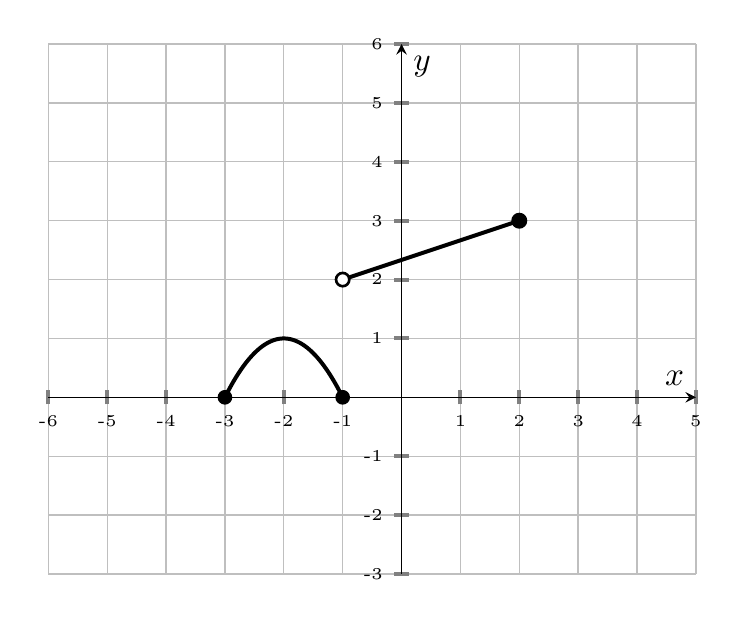
\begin{tikzpicture}[scale=1.2]
			\begin{axis}[
			axis lines=middle,
			unit vector ratio=1 1 1,
			grid=major,
			xmin=-6,
			xmax=5,
			ymin=-3,
			ymax=6,
			xlabel=$x$,
			ylabel=$y$,
			tick label style={font=\tiny},
			xtick={-6,-5,-4,...,5},
			xticklabels={-6,-5,-4,-3,-2,-1, ,1,2,3,4,5},
			ytick={-3,-2,...,2,3,4,5,6},
			yticklabels={-3,-2,-1, ,1,2,3,4,5,6},
			tick style={very thick},
			legend style={
				at={(rel axis cs:0,1)},
				anchor=north west,draw=none,inner sep=0pt,fill=gray!10}
			]
			\addplot[-,black,very thick,samples=100,domain=-3:-1]{-(x+2)^2+1};
			\addplot[incl] coordinates {(-3,0)};
			\addplot[incl] coordinates {(-1,0)};
			\addplot[-,black,very thick,samples=100,domain=-1:2]{3+(x-2)/3};
			\addplot[excl,thick] coordinates {(-1,2)};
			\addplot[incl,thick] coordinates {(2,3)};
			\end{axis}
			\end{tikzpicture}
\end{center}

\begin{subproblems}
\item State the domain of $G$. \hfill \underline{\hspace{2in}} \\
  \vfill
\item State the range of $G$. \hfill \underline{\hspace{2in}} \\
  \vfill
\item \textbf{Estimate} $G(0)$. \hfill \underline{\hspace{2in}} \\
  \vfill
\item For which $x$-value does $G(x)=1$? \hfill \underline{\hspace{2in}} \\
  \vfill
\item Graph the transformed function $G(x-3)+2$ on the axes above. \\
  \vfill
\end{subproblems}

\end{document}
%%% Local Variables:
%%% mode: LaTeX
%%% TeX-master: t
%%% End:
